\documentclass[10pt,a4paper]{article}
\usepackage{arabtex}
\usepackage[OT1,T1,LFE,LAE]{fontenc}
\usepackage[utf8]{inputenc}
\usepackage[arabic,english,farsi]{babel}
\usepackage{amsmath,amsfonts} % Math packages
\usepackage{amssymb}
%\usepackage{cmap}

\usepackage{multicol}

\usepackage{graphicx}
\usepackage[caption=false]{subfig}
\usepackage{color}
\usepackage{float}
\usepackage{sidecap}
%\sidecaptionvpos{figure}{c}
\usepackage{anysize}
\marginsize{2cm}{2cm}{2cm}{2cm}

\usepackage{listings}

\usepackage{appendix}
%\renewcommand{\appendixname}{Apéndices}
%\renewcommand{\appendixtocname}{Apéndices}
%\renewcommand{\appendixpagename}{Apéndices} 

\usepackage[colorlinks=true,plainpages=true,citecolor=blue,linkcolor=blue,urlcolor=cyan]{hyperref}
%\usepackage{hyperref}


%%% Equation and float numbering
\numberwithin{equation}{section}
\numberwithin{figure}{section}
\numberwithin{table}{section}


\newcommand{\horrule}[1]{\rule{\linewidth}{#1}}    % Horizontal rule

\newcommand{\titleText}{TCP and its Applications \\ Laboratory Manual}

\title{
\normalsize In the name of Allah\\
\vspace{10pt}
\LARGE\FR{بسم \allah الرحمن الرحیم}
\vspace{10pt}
\begin{center}
    %	\newcommand{\HRule}{\rule{\linewidth}{0.5mm}}
    \begin{minipage}{0.48\textwidth}
        \begin{flushleft}
            
\includegraphics[height=64pt,width=64pt]{../img/logo.png}
        \end{flushleft}
    \end{minipage}
    \begin{minipage}{0.48\textwidth}
        \begin{flushright}
            
\includegraphics[height=64pt]{../img/eng-logo.png}
        \end{flushright}
    \end{minipage}
\end{center}
\vspace*{-64pt}
%	\horrule{0.5pt} \\[0.4cm]
\huge \titleText\\
\vspace{40pt}
%	\horrule{2pt} \\[0.5cm]
}
\author{
\huge University of Tehran\\
\LARGE \FR{دانشگاه تهران}\\
\\
\LARGE School of Electrical and Computer Engineering\\
\FR{دانشکده مهندسی برق و کامپیوتر}\\
\\
\Large Computer Network Lab\\
\FR{آزمایشگاه شبکه‌های کامپیوتری}\\
\\
\\
\\
\normalfont
Dr. Ahmad Khonsari - \FR{احمد خونساری}\\
\href{mailto:a_khonsari@ut.ac.ir}{a\_khonsari@ut.ac.ir}\\
\\
\normalsize
Amir Haji Ali Khamseh'i - \FR{امیر حاجی علی خمسه‌ء}\\
\href{mailto:khamse@ut.ac.ir}{khamse@ut.ac.ir}\\
\\
\normalsize
Sina Kashi pazha - \FR{سینا کاشی پزها}\\
\href{mailto:sina\_kashipazha@ut.ac.ir}{sina\_kashipazha@ut.ac.ir}\\
\\
\normalsize
Mohammad Ali Shahsavand - \FR{محمد علی شاهسوند}\\
\href{mailto:mashahsavand@ut.ac.ir}{mashahsavand@ut.ac.ir}\\
\\
\normalsize
Amirahmad Khordadi - \FR{امیر احمد خردادی}\\
\href{mailto:a.a.khordadi@ut.ac.ir}{a.a.khordadi@ut.ac.ir}
}

\date{\vspace{30pt}\today\\\vspace{10pt}{\selectlanguage{farsi}\today}}

\usepackage{fancyhdr}
\pagestyle{fancy}
%\pagestyle{fancyplain}
\fancyhf{}
\fancyhead[L]{\footnotesize Computer Network Lab \\ \FR{آزمایشگاه شبکه‌های کامپیوتری}}
\fancyhead[R]{\footnotesize \titleText}
\fancyfoot[R]{\footnotesize School of Electrical and Computer Engineering\\\FR{دانشکده مهندسی برق و کامپیوتر}}
\fancyfoot[C]{\thepage}
\fancyfoot[L]{\footnotesize University of Tehran \\ \FR{دانشگاه تهران}}
\renewcommand{\footrulewidth}{0.8pt}
\renewcommand{\headrulewidth}{1pt}            % Remove header underlines
\renewcommand{\footrulewidth}{1pt}                % Remove footer underlines
\setlength{\headheight}{13.6pt}


\begin{document}
    \selectlanguage{english}

    %\vspace*{-1.5cm}
    \maketitle

    %\tableofcontents

    \pagebreak
    %Arabic \AR{\allah}
    %Persian \FR{فروشگاه}
    %Arabic \foreignlanguage{arabic}{كحض}
    %Persian \foreignlanguage{farsi}{فروشگاه}



    %	يعود تاريخ علوم الحاسوب إلى
    %\chapter
    %\section
    %\subsubsection
    %\subsection
    %\section
    %\chapter
    %\part
    %\caption
    %\end{otherlanguage}

    \section{HTTP Server}
    Study the Apache server configuration file (see Section 8.2.3).
    Examine the various configuration directives used and the corresponding settings. \\
    Start the Apache server on your host.
    In order to check if the server is working properly, you may start a \texttt{Mozilla} web browser to download the test page at \texttt{http://localhost/}.
    Then, execute \textbf{pgrep httpd} to list the process IDs of the \textbf{httpd} processes started.
    Save the output and the configuration file for the lab report.
    \subsection*{Report}
    \begin{enumerate}
        \item How many httpd processes were started?
        Which one was the master server, and which ones were the child servers?
        Justify your answer using the \texttt{httpd.conf} file. \\
        \item What is the purpose of initiating multiple httpd processes? \\
    \end{enumerate}

    %\pagebreak
    \section*{HTTP Request}
    Execute \textbf{wireshark} to capture packets between your host and a remote host. \\
    Login to the remote host’s web server: \textbf{telnet} \texttt{10.0.0.2} \textbf{80}. \\
    In the login console, type the following HTTP request line by line: \\
    \begin{verbatim}
        GET /usage/index.html HTTP/1.0
        From: guest@your host
        User-Agent: HTTPTool/1.0
    \end{verbatim}
    Note that you need to type the \texttt{Return} key to input the last line, which is blank.
    When the \textbf{telnet} process is terminated, save the output for your lab report. \\
    Terminate \textbf{wireshark} and analyze the captured HTTP packets.
    Print and save the HTTP request and response. \\
    Save the HTTP response’s data part into a file, named \texttt{index.html}.
    Use \texttt{Mozilla} to view the file.
    \subsection*{Report}
    \begin{enumerate}
        \item Submit the HTTP request and response, including the start-lines and all the headers.
    \end{enumerate}

    %\pagebreak
    \section*{HTTP Keep-Alive}
    By default, Apache server supports persistent connections. Before this exercise, the lab instructor should check the \texttt{KeepAlive} directive in the server configuration file to make sure it is turned on, as \texttt{KeepAlive} on. \\
    Execute \textbf{wireshark} to capture packets between your host and a remote host. \\
    Start \texttt{Mozilla} on your host. Go to menu \texttt{Edit/Preferences/Advanced/HTTP Networking}, and uncheck the Enable \texttt{Keep-Alive} checkbox to disable persistent connections. \\
    Enter the URL \texttt{http://10.0.0.2/try1.html}, to download the HTML file consisting a line of text, an embedded picture, and a hyperlink.
    Use \textbf{wireshark} and print the HTTP requests and responses for the lab report. \\
    Restart the \textbf{wireshark} program. Goto \texttt{Mozilla} menu \texttt{Edit/Preferences/Advanced/HTTP Networking}, and enable persistent connections by checking Enable \texttt{Keep-Alive}. \\
    Use \texttt{Mozilla} to reload the \texttt{try1.html} file. \\
    Use \textbf{wireshark} and print the HTTP requests and responses for the lab report.

    \subsection*{Report}
    \begin{enumerate}
        \item When you browsed the \texttt{try1.html} file for the first time, how many HTTP requests were sent?
        Which files were requested?
        How many TCP connections were used?
        \item Answer the above questions for when you browsed the \texttt{try1.html} file for the second time.
        \item What is the purpose of using persistent connections?
    \end{enumerate}

    %\pagebreak
    \section*{HTTP Submit}
    Execute \textbf{wireshark} to capture packets between your host and a remote host. \\
    Use \texttt{Mozilla} to download the \texttt{http://remote host/try2.htm} file, which is an \texttt{HTML} form, from the remote host. \\
    Fill a text string, e.g., the name of the host being used, into the text field in the form and click the submit button in the form. \\
    When the server response is received, terminate \textbf{wireshark}. \\
    Examine how CGI works, and identify the data string sent to the server.
    Save the HTTP request containing the data string for lab report.

    \subsection*{Report}
    \begin{enumerate}
        \item Submit the data string sent to the server.
    \end{enumerate}


    %\pagebreak
    \section*{DHCP \footnote{For the exercises in this section, we use the same network setting as the one used in the previous section.}}
    In this exercise, we use \texttt{guchi} as the DHCP server, with a configuration file shown in Table 8.3. Do the following.
    \begin{enumerate}
        \item Start the DHCP server on \texttt{guchi} in the foreground and working in the debugging mode: \textbf{/usr/sbin/dhcpd -d -f}.
        \item Execute \textbf{wireshark} to capture the DHCP messages in the network segment.
        \item Then do the following to enable DHCP for the Ethernet interface on \texttt{shakti}. \\
        Go to the system menu: \texttt{System Settings/Network}. In the \texttt{Network Configuration} dialog, choose the \texttt{Device} tab, and click on the \texttt{eth0} item. Next,click the Edit button to bring up the \texttt{Ethernet Device} dialog. In this dialog, check \texttt{Automatically obtain IP address settings with} and select \texttt{dhcp} from the following drop list. When the configuration is done, save the new configuration and then execute \textbf{/etc/init.d/network restart} to load the new configuration. \\
        When \texttt{shakti} is successfully reconfigured, execute \textbf{ifconfig -a} to display its network interface configurations and execute \textbf{netstat -rn} to display its routing table.
        Save the outputs for the lab report.
        \item Then, repeat 3 for \texttt{vayu}.
        \item Repeat 3 for agni.
        \item Repeat 3 for apah.
    \end{enumerate}
    Terminate \textbf{wireshark}.Print out the DHCP messages for the lab report. \\
    Save the DHCP server output on \texttt{guchi} for the lab report.

    \subsection*{Report}
    \begin{enumerate}
        \item Compare the DHCP operation captured by \textbf{wireshark} and that shown by the DHCP server output.
        Explain how DHCP works.
        \item Did \texttt{shakti} and \texttt{vayu} successfully obtain a set of new parameters?
        Compare the ifconfig and netstat output with the parameters carried in the corresponding DHCP messages.
        \item Answer the above question for agni.
        Explain why agni failed.
        \item Answer the above question for apah.
        Explain why apah succeeded.
    \end{enumerate}

    %\pagebreak
    \section*{NTP exercises 1 \footnote{Before proceeding to the next exercise, reboot the hosts to restore their original configurations.}}
    Execute \textbf{date} to display the system time of your host. Display the manual page of \textbf{date}, and study its options and usages.
    Try the following \textbf{date} commands: \\
    \textbf{date -{}-date='2 days ago'} \\
    \textbf{date -{}-date='3 months 2 days'} \\
    \textbf{date -{}-set='+3 minutes'} \\
    \textbf{date -r file\_name}\\
    You can choose any file in the current directory for the \textit{file\_name} parameter.
    \subsection*{Report}
    \begin{enumerate}
        \item Submit the \textbf{date} outputs you saved.
        Explain the use of the commands.
    \end{enumerate}

    \section*{NTP exercises 2}
    While \textbf{wireshark} is running, execute \textbf{rdate -p} \textit{remote\_host} to display the system time of the remote machine.
    Repeat the above \textbf{rdate} command, but use the \textbf{-u} option.
    Save the \textbf{wireshark} outputs for the lab report.

    \subsection*{Report}
    \begin{enumerate}
        \item What port numbers were used by the remote machine?
        What port numbers were used by the local host?
        \item How many bytes of data were returned by the remote time server, both in the UDP case and in the TCP case?
        \item What TCP header options were used?
    \end{enumerate}

    \section*{NTP exercises 3}
    In this exercise, we start the NTP server daemon on \texttt{shakti} and use NTP to
    synchronize all the other hosts to \texttt{shakti}.
    Study the NTP configuration file \texttt{/etc/ntp.conf} in \texttt{shakti} and in your host.
    If you are using another machine, you can telnet to shakti and display the \texttt{/etc/ntp.conf} file in the telnet window.
    Start the NTP server on \texttt{shakti} by: \textbf{/etc/init.d/ntpd start}.
    To determine the status of the NTP server, use \textbf{/etc/init.d/ntpd status}.
    Use \textbf{wireshark} to capture packets between your host and \texttt{shakti}.
    Execute \textbf{ntpdate -d -v 128.238.66.100} to synchronize your host to \texttt{shakti}.
    Study the output of this command.
    Save the \textbf{ntpdate} and the \textbf{wireshark} outputs for the lab report.
    \subsection*{Report}
    \begin{enumerate}
        \item Which port does the NTP server use?
        Justify your answer using the \textbf{wireshark} output.
    \end{enumerate}

    \section*{NAT exercises 1 \footnote{For the exercises in this section, we use a network setting as shown in Fig. 8.7. The lower subnet is a private network where the hosts are assigned with the Class A addresses with the 10.0.0.0/8 prefix. The upper subnet represents the Internet. The hosts, i.e., shakti and vayu are assigned with public IP addresses. Router 1 is used as the stub router, which performs address or port translation for the private network.}}
    Connect the hosts and Router 1 as shown in Fig.
    8.7. Then set the IP address and the network mask of your host as shown in the figure.
    In addition, you need to add a default route in your host’s routing table, using the router interface on your subnet as the default router.
    One student should \textbf{telnet} to the router and configure the router as shown in Table 8.5. Note that there is a static translation that maps 10.0.0.7, or \texttt{guchi}, to 128.238.61.104.
    Login to the router, execute \textbf{write term} to display the current router configuration.
    Execute \textbf{show ip nat translations} in the \textit{Privileged EXEC} mode to display the translation table.
    Save both outputs for the lab report.

    \subsection*{NAT Router Configuration in Fig. 8.7}
    \begin{verbatim}
        ip nat pool mypool 128.238.61.102 128.238.61.103 netmask 255.255.255.0
        ip nat inside source list 8 pool mypool

        ip nat inside source static 10.0.0.7 128.238.61.104

        interface ethernet 0
        ip address 128.238.61.1 255.255.255.0
        ip nat outside

        interface ethernet 1
        ip address 10.0.0.1 255.0.0.0
        ip nat inside

        access-list 8 deny host 10.0.0.7
        access-list 8 permit 10.0.0.0 0.0.0.255
    \end{verbatim}
    \begin{figure}[H]
        \centering
        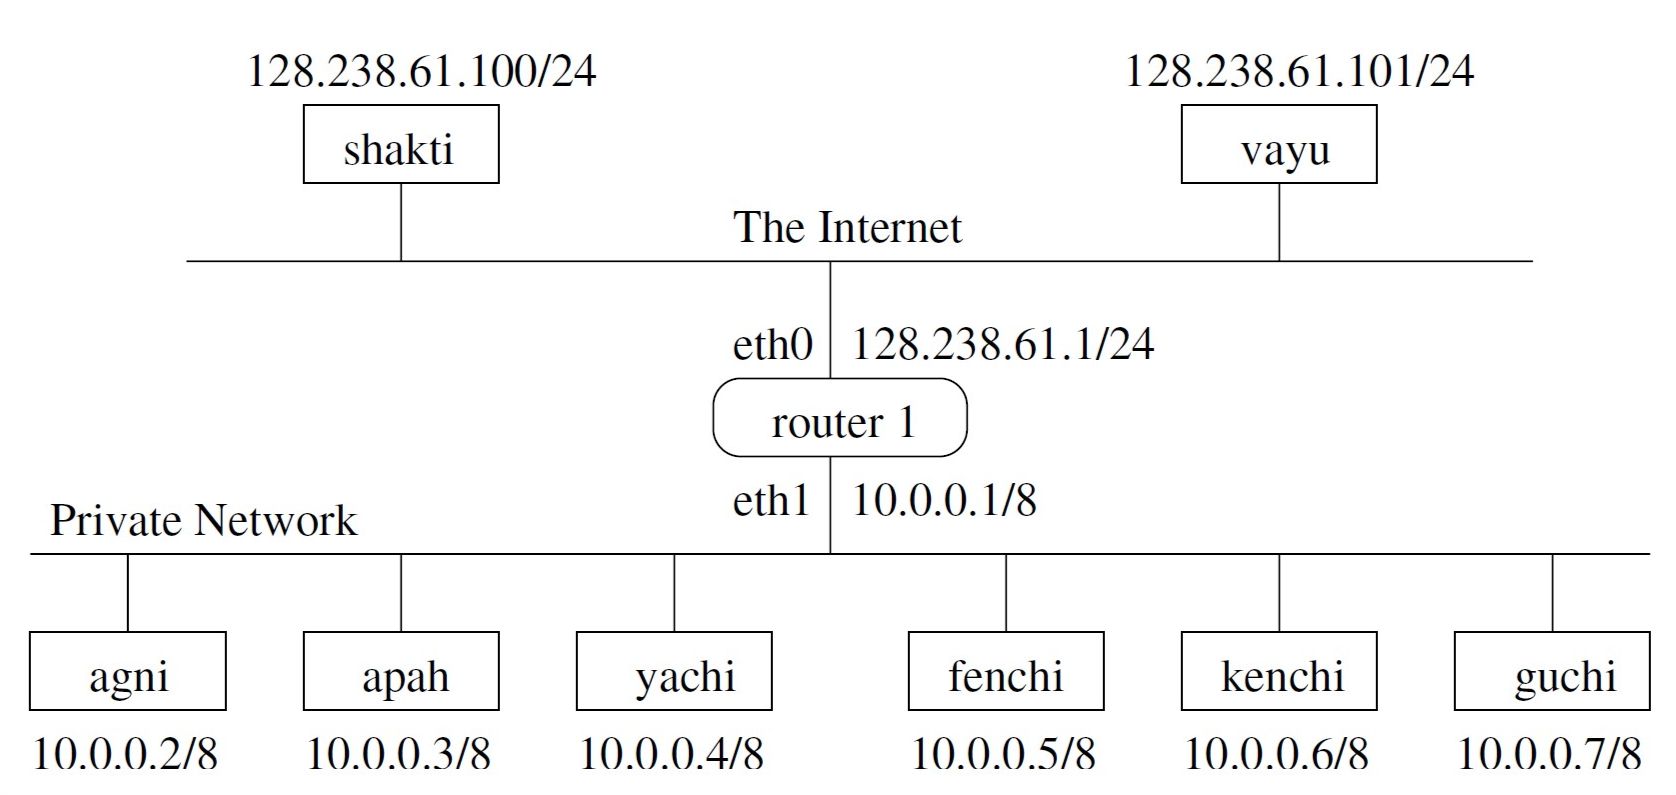
\includegraphics[width=\textwidth]{img/fig1.png}
    \end{figure}
    \subsection*{Report}
    \begin{enumerate}
        \item How many entries were there in the translation table?
        Why?
    \end{enumerate}

    \section*{NAT exercises 2}
    Keep the login session to the router running. Execute \textbf{wireshark} on all the hosts. \\
    Before any host in the private network send any packets out, ping an inside host (e.g., \texttt{fenchi}) from an outside host (e.g., \textbf{vayu}). You may try to ping 10.0.0.5, 128.238.61.102, 128.238.61.103, or 128.238.61.104. Can you ping these IP addresses? \\
    Let an inside host send packets to an outside host, e.g., from \texttt{fenchi}, execute ping 128.238.61.100. Can you ping \texttt{fenchi} from an outside host now? Why? Which IP address should be used in the ping command in order to ping \texttt{fenchi}? \\
    Execute show ip nat translations in the router login window to display the translation table. Save the output for the lab report. \\
    Exchange the data you saved with a student in the other subnet.
    \subsection*{Report}
    \begin{enumerate}
        \item Answer the above questions.
        Use the saved translation table to justify your answers.
        \item Compare the IP header of the ICMP query captured in the private network with that of the same ICMP query captured in the upper subnet, list their differences.
        Explain how NAT works.
        \item In addition to the IP address, what else was changed in the ICMP query packet?
    \end{enumerate}


    \section*{NAT exercises 3}
    Keep the login session to the router running. Execute \textbf{wireshark} to capture ICMP messages. \\
    Execute \textbf{sock -i -u -n1 128.238.61.101 8888} on \texttt{agni} to generate an ICMP port unreachable error. \\
    Print the ICMP error message for the lab report. \\
    Execute \textbf{show ip nat translations} in the router login window to display the translation table.
    Save the output for the lab report.
    Exchange the data you saved with a student in the other subnet.
    \subsection*{Report}
    \begin{enumerate}
        \item Analyze the IP headers, the ICMP headers, and the ICMP payloads of the ICMP port unreachable errors captured in the private network and in the public network from the first experiment.
        Explain how ICMP error was handled by the NAT router.
    \end{enumerate}

    \section*{NAT exercises 4}
    Reboot the router to restore its default configuration.
    Then, configure the router to use PAT, as given in Table 8.6. Now all the hosts in the private network use the same IP address 128.238.61.1. However, note that there is a static translation that maps guchi’s port 80 to 128.238.61.1 port 80. \\
    Execute \textbf{wireshark} on all the hosts. \\
    Generate traffic between the inside and outside hosts.
    Examine the \textbf{wireshark} output to see how PAT works.
    Start the Apache web server on \texttt{guchi}. Also, start the web browser \texttt{Mozilla} on an outside host (e.g., \texttt{shakti}), and enter the URL \texttt{http://128.238.61.1}. Save the \textbf{wireshark} output.
    Use \textbf{show ip nat translations} to display and then save the translation table.
    Exchange the data you saved with a student in the other subnet.
    \subsection*{PAT Router Configuration in Fig. 8.7}
    \begin{verbatim}
        ip nat inside source list 8 interface ethernet 0 overload

        ip nat inside source static tcp 10.0.0.7 80 128.238.61.1 80

        interface ethernet 0
        ip address 128.238.61.1 255.255.255.0
        ip nat outside

        interface ethernet 1
        ip address 10.0.0.1 255.0.0.0
        ip nat inside

        access-list 8 deny host 10.0.0.7
        access-list 8 permit 10.0.0.0 0.0.0.255
    \end{verbatim}
    \subsection*{Report}
    \begin{enumerate}
        \item From the \textbf{wireshark} data, explain how PAT worked, both for a dynamic translation and a static translation.
        With PAT, can you have two web servers in the private network?
        If not, why?
        If yes, explain how this can be done.
    \end{enumerate}

\iffalse
    \section*{Socket programming exercises 1}
    Examine the UDP socket programs \texttt{/home/guest/UDPserver.c} and \texttt{/home/guest/UDPclient.c} to learn how to write a UDP socket program.
    Compile the C programs using \texttt{gcc -o UDPserver UDPserver.c -lnsl} and \texttt{gcc -o UDPclient UDPclient.c -lnsl}. \\
    Start \textbf{wireshark} to capture packets from or to a remote host. \\
    On the remote host, start the UDP server by \textbf{UDPserver server\_port}.
    Then, start the UDP client on your host by \textbf{UDPclient remote\_host server\_port a\_message}.
    You may execute the UDP client program on other hosts to connect to the same UDP server.
    Terminate \textbf{wireshark}, examine its output and compare the output with the UDP server and client outputs.
    Repeat the above experiments, but now use the \texttt{TCPserver.c} and \texttt{TCPclient.c}.

    \section*{Socket programming exercises 2}
    Execute \textbf{man setsockopt} to display the various socket options and how to set them.
    Examine the \textbf{netspy} and \textbf{netspyd} source code in Appendix C.2 to see how to create a multicast socket and how to set the TTL value for the packets.

    \section*{Socket programming exercises 3}
    This is an optional exercise on socket programming.
    Or, it can be assigned as a take-home project for extra credits.
    Note that familiarity with C programming is required.
    \subsection*{PROBLEM}
    Examine the message exchanges of FTP. Write a FTP client program which takes a file name as input, and upload the file to a standard FTP server on a remote machine.
    \subsection*{HINTS}
    \begin{itemize}
        \item First you need to set up the control connection to Port 21 of the remote machine, using a TCP socket.
        \item When the control connection is established, you need to exchange FTP commands with the remote FTP server, as given in Table 5.1.
        \item You can first run \textbf{telnet remote\_host 21}, then type \textbf{help} to list all the FTP commands.
        Also, you can try the commands out in the \textbf{telnet} window, e.g.\  use \textbf{USER guest} to send the user ID and \textbf{PASS guest1} to send the password to the FTP server.
        To terminate the \textbf{telnet} session, type \textbf{QUIT}.
        \item In your program, these messages should be sent to the FTP server by calling the \textbf{send()} function of the local TCP socket.
        \item Also your program needs to parse the server responses (some examples are given in Table 5.2) to find out the status of the previous FTP command.
        \item The FTP data connection should be established using the \textbf{PORT} command (see Chapter 5).
    \end{itemize}
\fi

\end{document}